\documentclass[border=10pt,tikz]{standalone}
\usepackage{tikz}
\usetikzlibrary{positioning,arrows.meta}
\begin{document}
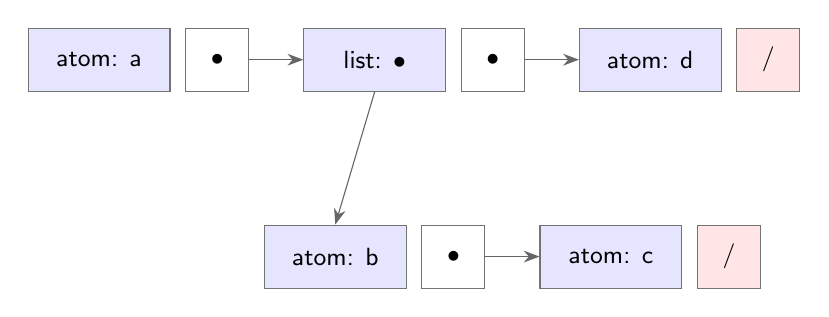
\begin{tikzpicture}[
  font=\sffamily\small,
  cell/.style={rectangle, draw=black!55, line width=0.4pt, minimum height=8mm,
               minimum width=18mm, inner sep=2pt, fill=blue!10, align=center},
  ptr/.style={cell, fill=white, minimum width=8mm},
  null/.style={cell, fill=red!10, minimum width=8mm},
  arr/.style={-{Stealth[length=2mm]}, draw=black!60}
]
% top row
\node[cell] (a1) at (0,    0) {atom: a};
\node[ptr]  (a1p) at (1.5, 0) {$\bullet$};

\node[cell] (l1)  at (3.5, 0) {list: $\bullet$};
\node[ptr]  (l1p) at (5.0, 0) {$\bullet$};

\node[cell] (d1)  at (7.0, 0) {atom: d};
\node[null] (d1p) at (8.5, 0) {/};

\draw[arr] (a1p.east) -- (l1.west);
\draw[arr] (l1p.east) -- (d1.west);

% second row (sublist of l1)
\node[cell] (b1)  at (3.0, -2.5) {atom: b};
\node[ptr]  (b1p) at (4.5, -2.5) {$\bullet$};
\node[cell] (c1)  at (6.5, -2.5) {atom: c};
\node[null] (c1p) at (8.0, -2.5) {/};

\draw[arr] (l1.south) -- (b1.north);
\draw[arr] (b1p.east) -- (c1.west);
\end{tikzpicture}
\end{document}
